%%%%%%%%%%%%%%%%%%%%%%%%%%%%%%%%%%%%%%%%%%%%%%%%%%%%%%%%%%%%%%%%%%%%%%%%%%%%%%%
%% 3.- PROGRAMA UTA
%%%%%%%%%%%%%%%%%%%%%%%%%%%%%%%%%%%%%%%%%%%%%%%%%%%%%%%%%%%%%%%%%%%%%%%%%%%%%%%

\cleardoublepage
\chapter{Programa Unidad de Tratamiento de Aire}
\chaptermark{Programa Unidad de Tratamiento de Aire}

\label{chap:anexoProgramaUTA} % etiqueta para poder referenciar luego en el texto con ~\ref{sec:intro}
% \addcontentsline{toc}{chapter}{Introducción, Objetivos, Metodología y Planificación

El programa para el control de la UTA se ha realizado el software ISaGRAF, que emplea los lenguajes de estándar IEEXXX:                   

\begin{itemize}
    \item Ventilación
    \item Filtrado
    \item Control de temperatura
    \item Control de humedad
\end{itemize}

El programa se compone de una parte de configuración de entradas, salidas, parámetros, alarmas y warnings, y otra parte dedicada a la programación del funcionamiento de la UTA.

En este anexo se muestran las variables configuradas (\hyperref[tab:variablesUTA]{Tabla~\ref{tab:variablesUTA}}), y la lógica de funcionamiento del programada.

\begin{center}
    \begin{longtable}{|p{3cm}|p{4cm}|p{7.5cm}|}
    \caption{Variables configuración control} \label{tab:variablesUTA} \\
    
    \hline \cellcolor{lightgray}\centering\textbf{GRUPO} & \cellcolor{lightgray}\centering\textbf{VARIABLE} & \cellcolor{lightgray}\textbf{DESCRIPCIÓN} \\ \hline 
    \endfirsthead
    
    \multicolumn{3}{c}%
    {{\bfseries \tablename\ \thetable{} ...continuación de la página anterior.}} \\
    \hline \cellcolor{lightgray}\textbf{GRUPO} & \cellcolor{lightgray}\textbf{PARÁMETRO} & \cellcolor{lightgray}\textbf{DESCRIPCIÓN} \\ \hline 
    \endhead
    
    \hline  \multicolumn{3}{c}%
    {{\bfseries \tablename\ \thetable{} continua en la página siguiente...}} \\
    \endfoot
    
    \hline
    \endlastfoot
    
        \centering{Entradas} & \small\centering\textbf{CNF01} & \small{Habilitar módulos de expansión (DIN4/DIN10)} \\ \cline{2-3}
        \centering{analógicas}& \small\centering\textbf{HUM01} & \small{Establecer consigna de humedad en \%HR} \\ \cline{2-3}
        & \small\centering\textbf{HUM02} & \small{Establecer banda para control de humedad, en \%HR} \\ \hline

        \centering{Entradas} & \small\centering\textbf{CNF01} & \small{Habilitar módulos de expansión (DIN4/DIN10)} \\ \cline{2-3}
        \centering{digitales} & \small\centering\textbf{HUM01} & \small{Establecer consigna de humedad en \%HR} \\ \cline{2-3}
        & \small\centering\textbf{HUM02} & \small{Establecer banda para control de humedad, en \%HR} \\ \hline

        \centering{Salidas} & \small\centering\textbf{CNF01} & \small{Habilitar módulos de expansión (DIN4/DIN10)} \\ \cline{2-3}
        \centering{digitales} & \small\centering\textbf{HUM01} & \small{Establecer consigna de humedad en \%HR} \\ \cline{2-3}
        & \small\centering\textbf{HUM02} & \small{Establecer banda para control de humedad, en \%HR} \\ \hline

        \centering{Salidas} & \small\centering\textbf{CNF01} & \small{Habilitar módulos de expansión (DIN4/DIN10)} \\ \cline{2-3}
        \centering{analógicas} & \small\centering\textbf{HUM01} & \small{Establecer consigna de humedad en \%HR} \\ \cline{2-3}
        & \small\centering\textbf{HUM02} & \small{Establecer banda para control de humedad, en \%HR} \\ \hline

        \centering{Alarmas} & \small\centering\textbf{CNF01} & \small{Habilitar módulos de expansión (DIN4/DIN10)} \\ \cline{2-3}
        & \small\centering\textbf{HUM01} & \small{Establecer consigna de humedad en \%HR} \\ \cline{2-3}
        & \small\centering\textbf{HUM02} & \small{Establecer banda para control de humedad, en \%HR} \\ \hline

        \centering{Warnings} & \small\centering\textbf{CNF01} & \small{Habilitar módulos de expansión (DIN4/DIN10)} \\ \cline{2-3}
        & \small\centering\textbf{HUM01} & \small{Establecer consigna de humedad en \%HR} \\ \cline{2-3}
        & \small\centering\textbf{HUM02} & \small{Establecer banda para control de humedad, en \%HR} \\ \hline
    \end{longtable}
\end{center}


\begin{figure}[H]
    \centering
    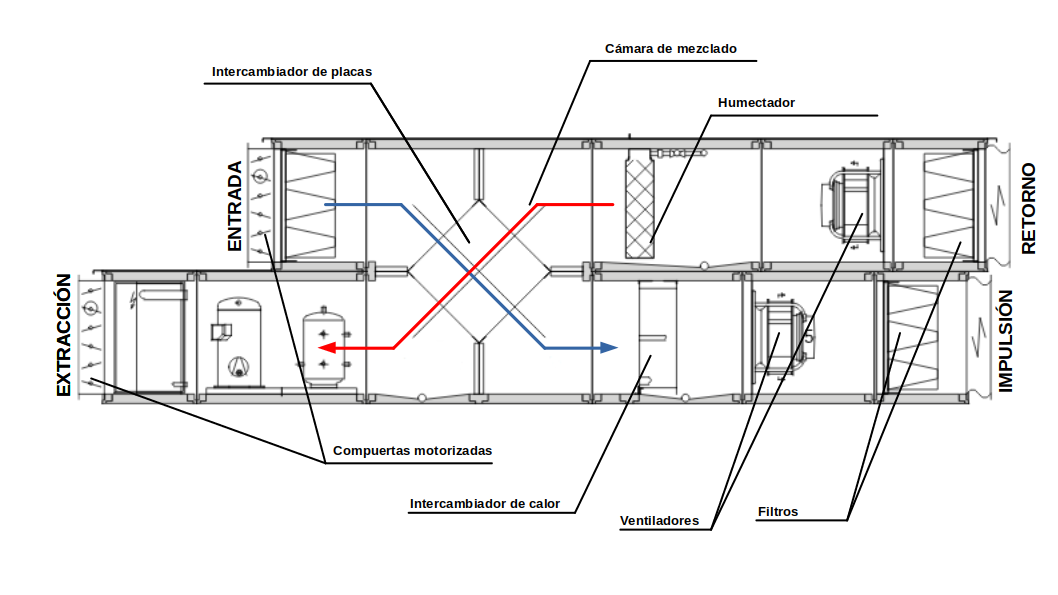
\includegraphics[width=\textwidth, keepaspectratio]{img/esquemaUTA}
    \caption{Plano de partes de una UTA}
    \label{figura:sasssssd}
\end{figure}
